\documentclass{standalone}
\usepackage{tikz}
\usetikzlibrary{arrows.meta, decorations.pathmorphing}

\begin{document}

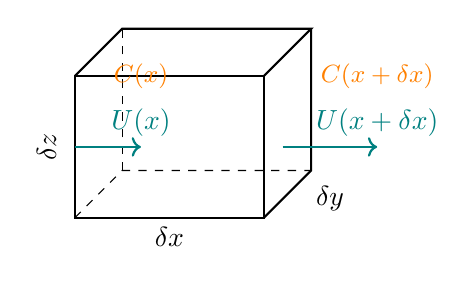
\begin{tikzpicture}[scale=1.2]

  % Define cube coordinates
  \coordinate (A) at (0,0);
  \coordinate (B) at (2,0);
  \coordinate (C) at (2,1.5);
  \coordinate (D) at (0,1.5);
  \coordinate (E) at (0.5,0.5);
  \coordinate (F) at (2.5,0.5);
  \coordinate (G) at (2.5,2);
  \coordinate (H) at (0.5,2);

  % Draw front face
  \draw[thick] (A) -- (B) -- (C) -- (D) -- cycle;
  % Draw top face
  \draw[thick] (D) -- (H) -- (G) -- (C);
  % Draw side face
  \draw[thick] (B) -- (F) -- (G);
  % Draw bottom face
  \draw[dashed] (A) -- (E) -- (F);
  % Draw back edges
  \draw[dashed] (E) -- (H);
  \draw[thick] (F) -- (G);

  % Dimension labels
  \node at (1.0,-0.2) {$\delta x$};
  \node[rotate=90] at (-0.3,0.75) {$\delta z$};
  \node at (2.7,0.2) {$\delta y$};


  % draw arrow at the right-hand face and label $U(x+\delta x)$
    \draw[->, teal, thick] (2.2,0.75) -- (3.2,0.75) node[right, above] {$U(x+\delta x)$};
    \draw[->, teal, thick] (-0.0,0.75) -- (0.7,0.75) node[left, above] {$U(x)$};
    % Label C(x) and C(x+dx) above the other labels
    \node[orange] at (3.2,1.5) {\small $C(x+\delta x)$};
    \node[orange] at (0.7,1.5) {\small $C(x)$};

\end{tikzpicture}

\end{document}
